\documentclass{beamer}
\usetheme{Madrid}
\usepackage[spanish]{babel}

\usepackage{tikz}

% Esto crea la portada de cada section
\AtBeginSection[]{
  \begin{frame}[plain]
  \begin{tikzpicture}[remember picture,overlay]
    \fill[structure.fg] (current page.south west) rectangle (current page.north east);
    \node at (current page.center) {
\Huge\color{white}\textbf{\insertsection}
    };
  \end{tikzpicture}
  \end{frame}
}

\title{Fuzzy Countries}
\author{Javier Comyn, Diego Fogued y Francisco J. González}
\institute{Universidad Politécnica de Madrid}
\date{Curso 2023/2024}

% Define a command to set the author for each slide
\newcommand{\slideauthor}[1]{\def\insertslideauthor{#1}}
\newcommand{\insertslideauthor}{}

% Set color for footline
\setbeamercolor{author in head/foot}{fg=white, bg=blue}

% Customize the footline
\setbeamertemplate{footline}
{
    \leavevmode%
    \hbox{%
    \begin{beamercolorbox}[wd=.4\paperwidth,ht=2.25ex,dp=1ex,left]{author in head/foot}%
        \usebeamerfont{author in head/foot}\insertshortauthor\hspace*{2em}
    \end{beamercolorbox}%
    \begin{beamercolorbox}[wd=.6\paperwidth,ht=2.25ex,dp=1ex,right]{title in head/foot}%
        \usebeamerfont{title in head/foot}\insertshorttitle\hspace*{2em}
    \end{beamercolorbox}}%
    \vskip0pt%
}

\begin{document}
\frame{\titlepage}

\begin{frame}
\frametitle{Índice de contenidos}
\tableofcontents
\end{frame}

\section{Introducción}
\begin{frame}
\frametitle{Background y Motivación}

\begin{itemize}
    \item Motivación: Mejorar la comprensión y modelado de las complejas dinámicas socioeconómicas de los países.
    \item Problema: Los modelos económicos tradicionales tienen dificultades con las incertidumbres y vaguedades de los datos reales.
    \item Solución: Utilizar la teoría de la lógica difusa para manejar estas incertidumbres.
    \item Objetivo: Crear un modelo socioeconómico más preciso y fiable, compararlo con datos reales para garantizar su credibilidad.
    \item Selección del Proyecto:
    \begin{itemize}
        \item Criterios: Fascinante, desafiante, adecuado a los principios de la lógica difusa, aplicable a la vida real.
        \item Consideración Inicial: Análisis psicológico o salud mental humana.
        \item Elección Final: Analizar la relación entre indicadores socioeconómicos y ambientales y la felicidad de la población.
    \end{itemize}
\end{itemize}

\end{frame}
\begin{frame}
\frametitle{Objetivos del Proyecto}
\begin{itemize}
    \item Objetivo Principal: Desarrollar un modelo socioeconómico que proporcione información sobre las condiciones económicas y ambientales.
    \item Visualización: Usar Uflese para visualizar los resultados y asegurar su comprensibilidad y utilidad.
    \item Credibilidad: Establecer un modelo creíble que ofrezca información valiosa.
    \item Enfoque:
    \begin{itemize}
        \item Desarrollar un sistema de lógica difusa con funciones y reglas.
        \item Analizar la relación entre indicadores socioeconómicos/ambientales y la felicidad de la población.
        \item Utilizar datos de fuentes reputadas como el Informe Mundial de la Felicidad y el Banco Mundial.
        \item Validar los resultados comparando las puntuaciones de felicidad obtenidas con las del Informe Mundial de la Felicidad.
    \end{itemize}
\end{itemize}

\end{frame}

\section{Marco teórico}
\begin{frame}
\frametitle{Marco teórico}
\begin{itemize}
    \item Definición: Lógica multievaluada donde los valores de verdad oscilan entre 0 y 1.
    \item Propósito: Manejar el concepto de \textit{fuzzy}, a diferencia de la lógica booleana con valores solo de 0 o 1.
    \item Extensión: Gestionar grados de verdad parcial con funciones específicas para variables lingüísticas.
\end{itemize}

\end{frame}

\section{Metodología}
\begin{frame}
\frametitle{Metodología}
\begin{itemize}
    \item \textbf{Recolección de Datos}
    \begin{itemize}
        \item Fuentes
    \end{itemize}
    \item \textbf{Descripción de los Datos}
    \begin{itemize}
        \item Análisis de las características de los datos recolectados.
    \end{itemize}
    \item \textbf{Preprocesamiento de Datos}
    \item \textbf{Diseño y Desarrollo de la Base de Datos}
    \item \textbf{Implementación del Sistema Difuso}
    \item \textbf{Resultados y Discusión}
    \item \textbf{Desafíos y Soluciones}
    \item \textbf{Conclusiones y Trabajo Futuro}

\end{itemize}
\end{frame}

\section{Diseño de la Base de Datos}
\begin{frame}
\frametitle{Recopilación}
\slideauthor{Javier Comyn}
\begin{itemize}
    \item Consultar fuentes: Banco Mundial, OMS, Kaggle...
    \item Escoger indicadores más relevantes para un análisis socioeconómico.
    \item Elección de los conjuntos de datos más confiables y actualizados.
    \item Asegurarse de la consistencia y veracidad.
\end{itemize}
\end{frame}
\begin{frame}
\frametitle{Descripción}
\slideauthor{Javier Comyn}
\begin{itemize}
    \item Índice de libertad económica
    \item Temperatura media (ºC)
    \item Tasa suicidios por 100.000 habitantes
    \item Percepción de la corrupción
    \item Densidad de población
    \item Porcentaje de terreno agrícola
    \item Superficie
    \item Tamaño del ejército
    \item Tasa de natalidad
    \item CO2
    \item Índice de Precios al Consumidor (IPC)
    \item Tasa de fertilidad
    \item Porcentaje de área forestal
\end{itemize}
\end{frame}
\begin{frame}
\frametitle{Descripción}
\slideauthor{Javier Comyn}
\begin{itemize}
    \item PIB per cápita
    \item Alumnos en educación primaria
    \item Alumnos en educación post-obligatoria
    \item Mortalidad infantil
    \item Esperanza de vida
    \item Tamaño de la población
    \item Población activa
    \item Ingresos fiscales (\% del PIB)
    \item Tasa de paro
    \item Población urbana
    \item Energías renovables
    \item Salario mínimo
    \item Edad media
\end{itemize}
\end{frame}
\begin{frame}
\frametitle{Preprocesamiento y Limpieza}
\slideauthor{Javier Comyn}
\begin{itemize}
    \item Integrar todas las variables en una única base de datos
    \item Eliminar inconsistencias
    \item Tratar valores faltantes
    \item Convertir todos los valores en enteros
\end{itemize}
\end{frame}

\section{Análisis de Datos}

\begin{frame}
\frametitle{Funciones Difusas}
\slideauthor{Javier Comyn}
Para cada variable, definimos una función difusa basándonos en nuestro propio criterio. Los valores se van ajustando progresivamente al ir probando y revisando cada una de ellas.
\vspace*{+5mm} % Ajusta este valor para cambiar el espacio entre las figuras
\begin{figure}
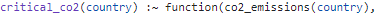
\includegraphics[width=\textwidth]{Images/co2_1.png} 
\end{figure}
\vspace*{-5mm} % Espacio entre figuras
\begin{figure}

\includegraphics[width=\textwidth]{Images/co2_2.png} 
\end{figure}
\end{frame}

\begin{frame}
\frametitle{Reglas Difusas}
\slideauthor{Javier Comyn}
\end{frame}

\begin{frame}
\frametitle{Consultas}
\slideauthor{Javier Comyn}
Fotos de consultas
%\begin{figure}
%\includegraphics[width=\textwidth]{ruta/a/tu/imagen.jpg} % Reemplaza 'ruta/a/tu/imagen.jpg' con la ruta a tu imagen
%\caption{Descripción de la imagen}
%\end{figure}
\end{frame}

\begin{frame}
\frametitle{Resultados Notables}
\slideauthor{Javier Comyn}
Fotos de consultas
\end{frame}

\section{Optimización}
\begin{frame}
\frametitle{Optimización}
\slideauthor{Autor 2}

\end{frame}

\section{Resultados y Conclusiones}
\begin{frame}
\frametitle{Resultados}
\slideauthor{Autor 2}
texto
\end{frame}

\end{document}
